\documentclass[border=10pt]{standalone}
%%%<
\usepackage{verbatim}
%%%>
\usepackage{pgfplots}
\pgfplotsset{width=7cm,compat=1.8}
\begin{comment}
:Title: Clipped Output Sine Wave Signal
:Tags: 2D;Clipping;Functions
:Author: Christian Feuersänger
:Slug: clipped-curve

A sine curve, where the y-values do not exceed a certain value.

PGFPlots has two different types of clipping: the first is the graphical
clipping operation which is activated by \clip, the second is based on
coordinate value manipulation, more precisely by restrict y to domain*.

This topic was discussed on:
http://latex-community.org/forum/viewtopic.php?f=45&t=22837
\end{comment}
% Create a function for generating inverse normally distributed numbers using the Box–Muller transform
\pgfmathdeclarefunction{invgauss}{2}{%
  \pgfmathparse{sqrt(-2*ln(#1))*cos(deg(2*pi*#2))}%
}
\newcommand*{\val}{0.8}% the absolut value of the limit
% Code for brownian motion
\begin{document}
  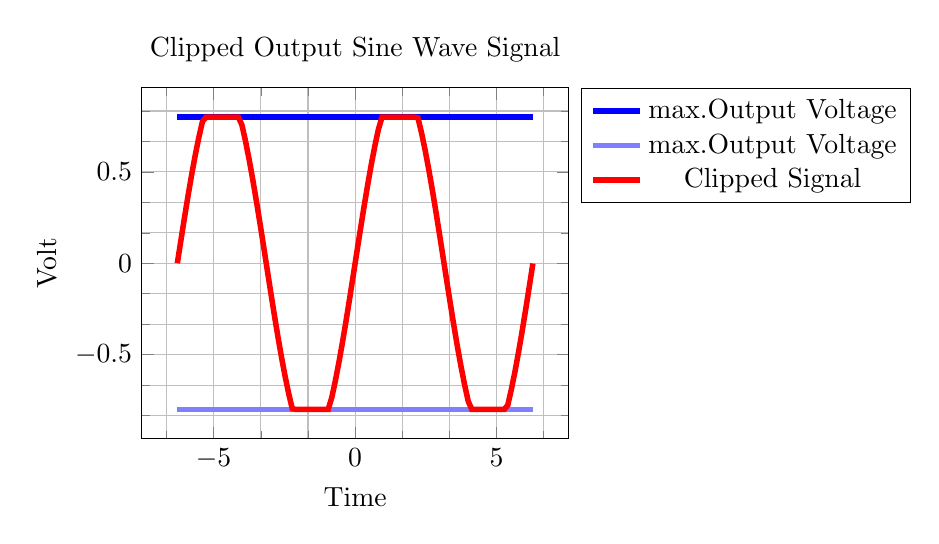
\begin{tikzpicture}
    \begin{axis}[
        domain     = -6.283:6.283,
        grid       = both, minor tick num=2,
        title      = Clipped Output Sine Wave Signal,
        xlabel     = Time,
        ylabel     = Volt,
        legend pos = outer north east,
        restrict y to domain* = -\val:\val
      ]
      \addplot[blue, line width=2pt] {\val};
      \addplot[blue!50, line width=2pt] {-\val};
      \addplot+[no marks, samples=100, red, line width=2pt] {sin(deg(x))};
      \legend{max.Output Voltage, max.Output Voltage, Clipped Signal}
    \end{axis}
  \end{tikzpicture}
\end{document}